%%%%%%%%%%%%%%%%%%%%%%%%%%%%%%%%%%%%%%%%%%%%%%
%%%%%%%%%%%%%%%%%%%%%%%%%%%%%%%%%%%%%%%%%%%%%%
%%                                          %%
%% Important note on usage                  %%
%% -----------------------                  %%
%% This file must be compiled with PDFLaTeX %%
%% Using standard LaTeX will not work!      %%
%%                                          %%
%%%%%%%%%%%%%%%%%%%%%%%%%%%%%%%%%%%%%%%%%%%%%%
%%%%%%%%%%%%%%%%%%%%%%%%%%%%%%%%%%%%%%%%%%%%%%

%% The '3p' and 'times' class options of elsarticle are used for Elsevier CRC
\documentclass[5p]{elsarticle}
% \documentclass[3p,times]{elsarticle}
% \documentclass[3p]{elsarticle}

\usepackage[american]{babel}
\usepackage{amsmath}
\usepackage[version=3]{mhchem} 
% \usepackage{fixltx2e}
% \usepackage{refcount}
% \usepackage{siunitx}
% \usepackage{lastpage}
% \usepackage{textcomp}
\usepackage{mathtools}

\usepackage{xfrac}
\usepackage{lmodern}
\usepackage[hidelinks]{hyperref}
% \usepackage{cool}
% \usepackage{cancel}
\usepackage{microtype}
\usepackage{listings}
\usepackage{mcode}
\usepackage [autostyle, english = american]{csquotes}
\usepackage{longtable}
\usepackage{subcaption}
\usepackage{booktabs,siunitx}
\usepackage{gensymb}
\usepackage[normalem]{ulem}

% \usepackage{mathtools, cuted}


% \usepackage[usenames,dvipsnames,svgnames,table]{xcolor}
\usepackage{color}

\usepackage[colorinlistoftodos]{todonotes}

\usepackage[section]{placeins}
\usepackage{multirow}


\lstset{basicstyle=\small\ttfamily,columns=fullflexible}

% \usepackage{verbatim}



% \usepackage{gensymb}
% \usepackage{enumerate}
% \usepackage{float}
% \usepackage{bm}
% \usepackage{csquotes}
% \usepackage{mathtools}
% \usepackage{natbib}
% \usepackage{biblatex}

%% The `ecrc' package must be called to make the CRC functionality available
\usepackage{ecrc}

%% The ecrc package defines commands needed for running heads and logos.
%% For running heads, you can set the journal name, the volume, the starting page and the authors

%% set the volume if you know. Otherwise `00'
\volume{00}

%% set the starting page if not 1
\firstpage{1}

%% Give the name of the journal
\journalname{Nuclear Instruments and Methods in Physics Research B}

%% Give the author list to appear in the running head
%% Example \runauth{C.V. Radhakrishnan et al.}
\runauth{A.S. Voyles et al.}

%% The choice of journal logo is determined by the \jid and \jnltitlelogo commands.
%% A user-supplied logo with the name <\jid>logo.pdf will be inserted if present.
%% e.g. if \jid{yspmi} the system will look for a file yspmilogo.pdf
%% Otherwise the content of \jnltitlelogo will be set between horizontal lines as a default logo

%% Give the abbreviation of the Journal.
\jid{nimb}
% \jid{yspmi}

%% Give a short journal name for the dummy logo (if needed)
\jnltitlelogo{Nucl Instrum Meth B}

%% Hereafter the template follows `elsarticle'.
%% For more details see the existing template files elsarticle-template-harv.tex and elsarticle-template-num.tex.

%% Elsevier CRC generally uses a numbered reference style
%% For this, the conventions of elsarticle-template-num.tex should be followed (included below)
%% If using BibTeX, use the style file elsarticle-num.bst

%% End of ecrc-specific commands
%%%%%%%%%%%%%%%%%%%%%%%%%%%%%%%%%%%%%%%%%%%%%%%%%%%%%%%%%%%%%%%%%%%%%%%%%%

%% The amssymb package provides various useful mathematical symbols
\usepackage{amssymb}
%% The amsthm package provides extended theorem environments
\usepackage{amsthm}

%% The lineno packages adds line numbers. Start line numbering with
%% \begin{linenumbers}, end it with \end{linenumbers}. Or switch it on
%% for the whole article with \linenumbers after \end{frontmatter}.
%% \usepackage{lineno}

%% natbib.sty is loaded by default. However, natbib options can be
%% provided with \biboptions{...} command. Following options are
%% valid:

%%   round  -  round parentheses are used (default)
%%   square -  square brackets are used   [option]
%%   curly  -  curly braces are used      {option}
%%   angle  -  angle brackets are used    <option>
%%   semicolon  -  multiple citations separated by semi-colon
%%   colon  - same as semicolon, an earlier confusion
%%   comma  -  separated by comma
%%   numbers-  selects numerical citations
%%   super  -  numerical citations as superscripts
%%   sort   -  sorts multiple citations according to order in ref. list
%%   sort&compress   -  like sort, but also compresses numerical citations
%%   compress - compresses without sorting
%%
%% \biboptions{comma,round}

% \biboptions{}

% if you have landscape tables
\usepackage[figuresright]{rotating}

% put your own definitions here:
%   \newcommand{\cZ}{\cal{Z}}
%   \newtheorem{def}{Definition}[section]
%   ...

% add words to TeX's hyphenation exception list
%\hyphenation{author another created financial paper re-commend-ed Post-Script}

% declarations for front matter

\usepackage{fancyvrb}
\usepackage{color}
 
\definecolor{mygreen}{rgb}{0,0.6,0}
\definecolor{mygray}{rgb}{0.5,0.5,0.5}
\definecolor{mymauve}{rgb}{0.58,0,0.82}

\lstset{ %
  backgroundcolor=\color{white},   % choose the background color
  basicstyle=\footnotesize,        % size of fonts used for the code
  breaklines=true,                 % automatic line breaking only at whitespace
  captionpos=b,                    % sets the caption-position to bottom
  commentstyle=\color{mygreen},    % comment style
  escapeinside={\%*}{*)},          % if you want to add LaTeX within your code
  keywordstyle=\color{blue},       % keyword style
  stringstyle=\color{mymauve},     % string literal style
}

% Sin and Cos with auto-parentheses 
\newcommand{\sinp}[1]{\sin{\left( #1\right)}}
\newcommand{\cosp}[1]{\cos{\left( #1\right)}}
\newcommand{\expp}[1]{\exp{\left( #1\right)}}
\newcommand{\sinhp}[1]{\sinh{\left( #1\right)}}
\newcommand{\lnp}[1]{\ln{\left( #1\right)}}
\newcommand{\pp}[1]{\left( #1\right)}
\newcommand{\sci}[2]{ #1 \cdot 10^{#2}\ }
\newcommand{\angstrom}{\mbox{\normalfont\AA}}
\newcommand{\norm}[1]{\lVert #1 \rVert}

\newcommand{\textred}[1]{\textcolor{red}{ #1}}
\newcommand{\redactedit}[1]{\textcolor{blue}{ \sout{#1}}}


\newcommand{\colornote}[1]{\textcolor{red}{ COMMENT\large\footnote{\textcolor{red}{#1}}}}

\newcommand{\comment}[1]{\todo[color=blue!20!white,inline]{ASV: #1}} 

% Tweak sim for better inline text tilde
\newcommand{\mytilde}{\raisebox{0.5ex}{\texttildelow}}
% \newcommand{\mytilde}{\raise.17ex\hbox{$\scriptstyle‌​\sim$}}

\sisetup{separate-uncertainty=true,table-space-text-post = *}

\newcommand{\minitab}[2][l]{\begin{tabular}{#1}#2\end{tabular}}

\newcommand{\subfigimg}[3][,]{%
  \setbox1=\hbox{\includegraphics[#1]{#3}}% Store image in box
  \leavevmode\rlap{\usebox1}% Print image
  \rlap{\hspace*{50pt}\raisebox{\dimexpr\ht1-2\baselineskip}{#2}}% Print label
  \phantom{\usebox1}% Insert appropriate spcing
}


\makeatletter
% Make common definition of mean
\newcommand*\mean[1]{\overline{#1\raisebox{3mm}{}}}

\makeatother


\begin{document}

\begin{frontmatter}

%% Title, authors and addresses

%% use the tnoteref command within \title for footnotes;
%% use the tnotetext command for the associated footnote;
%% use the fnref command within \author or \address for footnotes;
%% use the fntext command for the associated footnote;
%% use the corref command within \author for corresponding author footnotes;
%% use the cortext command for the associated footnote;
%% use the ead command for the email address,
%% and the form \ead[url] for the home page:
%%
\title{Measurement of nuclear excitation functions for proton induced reactions (E$_{\text{p}}$ = 40 -- 90 MeV) on Nb and Cu}

%% \tnotetext[label1]{}
%% \author{Name\corref{cor1}\fnref{label2}}
%% \ead{email address}
%% \ead[url]{home page}
%% \fntext[label2]{}
%% \cortext[cor1]{}
%% \address{Address\fnref{label3}}
%% \fntext[label3]{}

% \dochead{Short}
%% Use \dochead if there is an article header, e.g. \dochead{Short communication}


% \author[rvt]{C.V. ̃Radhakrishnan\corref{cor1}\fnref{fn1}}
\author[ucb]{A.S. Voyles \corref{cor1}}
\ead{andrew.voyles@berkeley.edu}

% \author[lbl]{M.S. Basunia}
% 
% \author[ucb]{J.C. Batchelder}
% 
% \author[llnl]{J.D. Bauer}
% 
% \author[geo]{T.A. Becker}


\author[ucb,lbl]{Lee A. Bernstein}


\author[lanl]{Eva R. Birnbaum}

\author[uwm]{Jonathan W. Engle}

\author[lanl]{Francois M. Nortier}

% \author[ucb]{M.A. Unzueta}
% 
% \author[ucb]{K.A. van Bibber}



%% use optional labels to link authors explicitly to addresses:
%% \author[label1,label2]{<author name>}
%% \address[label1]{<address>}
%% \address[label2]{<address>}

\cortext[cor1]{Corresponding author}
% \cortext[cor2]{Principal corresponding author}
% \fntext[fn1]{This is the specimen author footnote.}
% \fntext[fn2]{Another author footnote, but a little more longer.}

% \address[ucb]{Department of Nuclear Engineering, University of California, Berkeley, Etcheverry Hall, 2521 Hearst Ave, Berkeley, CA 94709}
% \address[lbl]{Lawrence Berkeley National Laboratory,  1 Cyclotron Rd, Berkeley, CA 94720}
% \address[llnl]{Lawrence Livermore National Laboratory, 7000 East Ave, Livermore, CA 94550}

\address[ucb]{Department of Nuclear Engineering, University of California, Berkeley, 4155 Etcheverry Hall, MC 1730, Berkeley, CA 94720, USA}
\address[lbl]{Lawrence Berkeley National Laboratory, 1 Cyclotron Rd., Berkeley, CA 94720, USA}
% \address[llnl]{Lawrence Livermore National Laboratory, Livermore CA, 94551 USA}
% \address[geo]{Berkeley Geochronology Center, Berkeley CA,  94709  USA}
\address[uwm]{Department of Medical Physics, University of Wisconsin -- Madison, 1111 Highland Ave., Madison, WI 53705, USA}
\address[lanl]{Los Alamos National Laboratory, P.O. Box 1663, Los Alamos, NM 87544, USA}




\begin{abstract}







XXXXX




% Cross sections for the \ce{^{47}Ti}(n,p)\ce{^{47}Sc} and \ce{^{64}Zn}(n,p)\ce{^{64}Cu} reactions have been measured for quasi-monoenergetic DD neutrons produced by the UC Berkeley High Flux Neutron Generator.
% The study was motivated by interest in the production of \ce{^{47}Sc} and \ce{^{64}Cu} as emerging medical isotopes.
% The cross sections were measured in ratio to the \ce{^{113}In}(n,n')\ce{^{113m}In} and \ce{^{115}In}(n,n')\ce{^{115m}In} inelastic scattering reactions on co-irradiated indium samples.
% Post-irradiation counting using an HPGe and LEPS detectors allowed for cross section determination to within 5\% uncertainty.
% The cross sections were determined with lower uncertainty than existing measurements and are found to be  in good agreement with both empirical and theoretical values.
% This work highlights the utility of using DD plasma-based neutron sources for a host of nuclear data measurements and potentially for the production of radionuclides for medical applications.

% \comment{Karl:  \enquote{Comment to engender some discussion.  I have a small concern here, reminiscent of what happened to our electron backstreaming paper in PRAB.  To be publishable, even in NIMB, there has to be a crisp research question resolved, or some innovation.  I think an angle that is missing here is that this is a new design of neutron generator, whose design maximizes the flux density (n/sec/cm2), although the total flux, while respectable, is not spectacular in itself.  This is Lee's recent mantra, and I now understand its significance.  Problematically, as Andrew has pointed out, we don't have the actual instrument paper published yet, so the thrust of the paper can't be too focused on the flux density issue, but a workable angle would be \enquote{given we have this new capability, this is an example of its power}.  Let me suggest Lee provide a sentence for the abstract, and a few sentences of text in the appropriate spot.}}

% \comment{The abstract is now nicely short and sweet, but should it be expanded at all?}



\end{abstract}

\begin{keyword}
%% keywords here, in the form: keyword \sep keyword
Nb+p \sep Cu+p \sep Niobium \sep Copper\sep Aluminum \sep Nuclear cross sections \sep Proton activation \sep Proton transport \sep Stacked target activation \sep Monitor foils \sep Medical isotope production \sep MCNP \sep  LANL

%% MSC codes here, in the form: \MSC code \sep code
%% or \MSC[2008] code \sep code (2000 is the default)

\end{keyword}

\end{frontmatter}

%%
%% Start line numbering here if you want
%%
% \linenumbers

% \listoftodos


%% main text 
\section{Introduction} \label{sec:intro}

% \comment{cite theranostic papers, etc}


XXXXXX  \cite{Updegraff2013}.


\section{Experimental methods and materials}\label{sec:experiment}



\subsection{Stacked-target design }\label{sec:target_design}

% \comment{Regex to replace all hard figure references with LaTeX cross-references  [F,f]igure[^s*}]     }

XXXXXX

% \begin{figure}
%     \centering
%         \centering
%         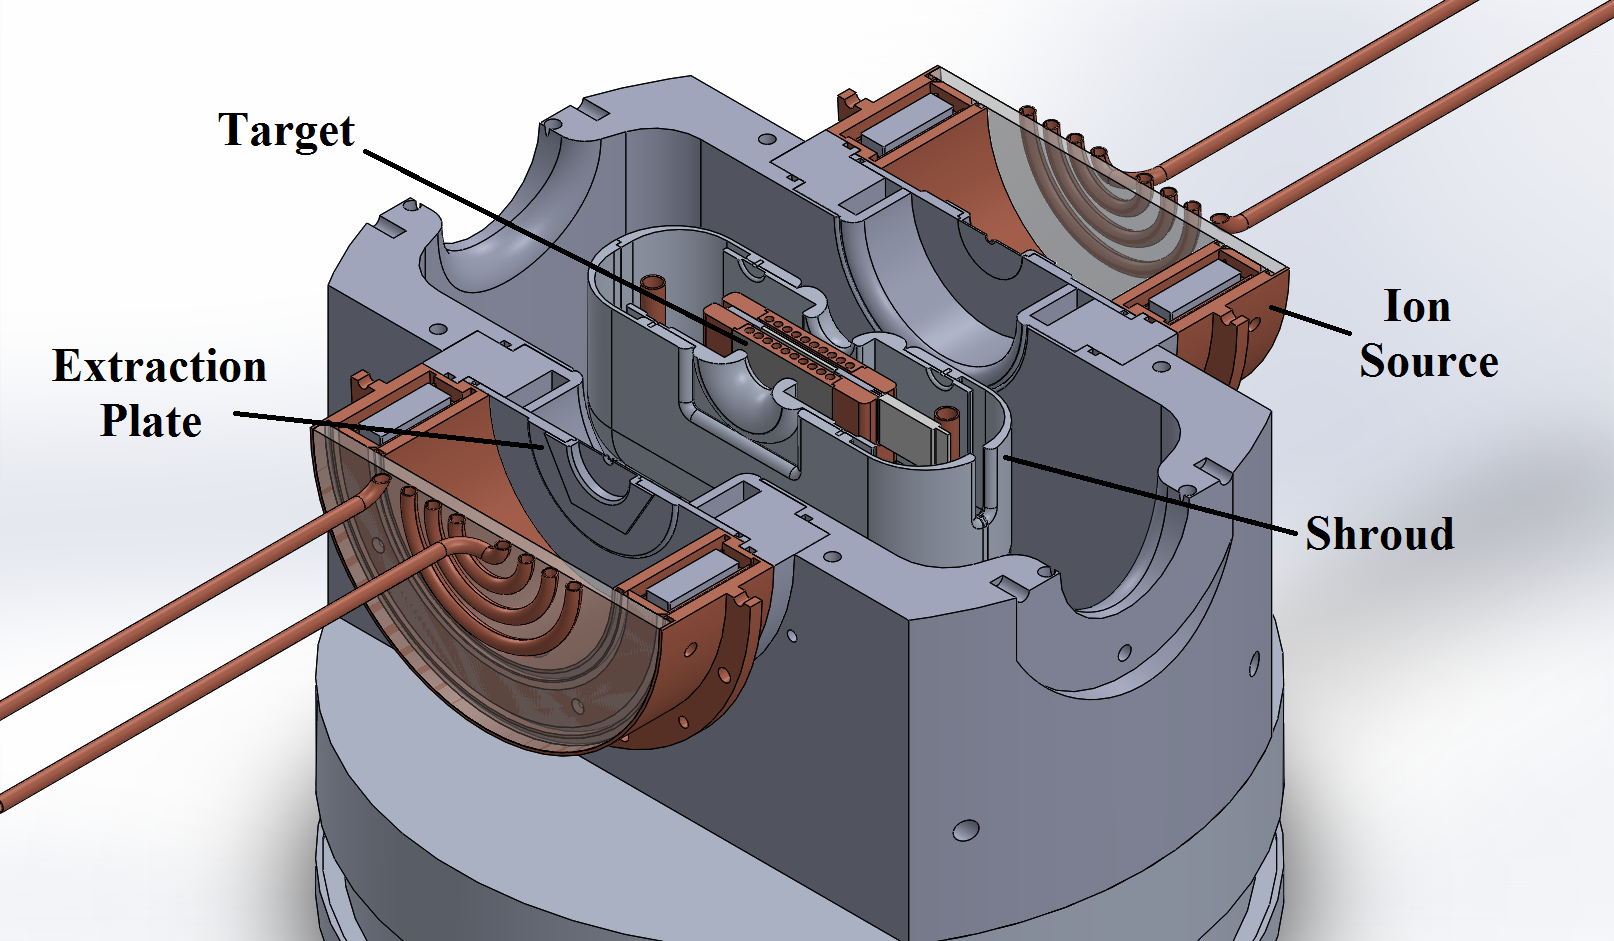
\includegraphics[height=2in]{./figures/cutaway.png}
%         \caption{Cut-away schematic of the HFNG. The ion source is approximately 20 cm in diameter.}
%                 \label{fig:hfng_b}
% \end{figure}



\subsection{Measurement of induced activities}\label{sec:spectroscopy}

XXXXXX



% \comment{Regex to replace table hard link with LaTeX cross-reference. - match w/ [T,t]able[^*}]   }


\subsection{Proton dosimetry}\label{sec:spectroscopy}

% describe integral equation for converting activities to currents here

XXXXXX


\subsection{Proton transport calculations}\label{sec:proton_transport}

XXXXXX

% \begin{equation}
% R = N_T \int_0^{E_{max}} \sigma(E) \dfrac{d\phi}{dE} dE
% \end{equation}







\subsection{Calculation of measured cross sections}\label{sec:calcs_sec}

%  include 1st and 2nd order bateman stuff here

XXXXXX

 

% \begin{align}
% N_{\gamma} &= N_D \epsilon_\gamma I_\gamma \\
% &=  \epsilon_\gamma I_\gamma  \dfrac{N_T \sigma\pp{\bar{E}} \phi\pp{\bar{E}} }{\lambda}\pp{1 - e^{-\lambda t_i}}  e^{-\lambda t_d} \pp{1 - e^{-\lambda t_c}} \nonumber
% \end{align}



% \autoref{eqn:single_xs_eqn} can be used to determine the unknown (n,p) cross sections relative to the well-known \ce{^{115}In}(n,n')\ce{^{115m}In} and \ce{^{113}In}(n,n')\ce{^{113m}In} inelastic scattering cross sections since the Zn and Ti samples were co-irradiated with indium foils.
% This approach has a number of advantages since the result is independent of neutron flux and only depends on the relative detector efficiencies at each gamma-ray energy.
 

\subsection{Systematic uncertainties}

XXXXXX




\section{Results}


XXXXXX

          
% \section{Discussion}




% XXXXXX
 
 
 
 \section{Conclusions}

XXXXXX


 
 \section{Acknowledgements}
 
 Stephen Graves - consulting for methodology, guidance.
 
%  We would like to particularly point out the crucial role played by Cory Waltz in the design and commissioning of the HFNG.
%  We wish to thank Marc Garland and Saed Mirzadeh for discussions regarding the use of neutron generators for isotope production.
%  We acknowledge Glenn Jones of G\&J Jones Enterprises of Dublin, CA for the construction  of the High Flux Neutron Generator. 
%  Lastly, we would like to acknowledge the students in the Nuclear Reactions and Radiation (NE102) laboratory course at UC Berkeley who participated in these experiments, including Joe Corvino, Nizelle Fajardo, Scott Parker and Evan Still.  
%  
%  This work has been carried out at the University of California, Berkeley, and performed under the auspices of the U.S. Department of Energy by Lawrence Livermore National Laboratory under contract \# DE-AC52-07NA27344 and Lawrence Berkeley National Laboratory under contract \# DE-AC02-05CH11231.
% Funding has been provided from the US Nuclear Regulatory Commission, the US Nuclear Data Program, the Berkeley Geochronology Center, NSF ARRA Grant \# EAR-0960138, the University of California Laboratory Fees Research Grant \# 12-LR-238745, and  DFG Research Fellowship \# RU 2065/1-1.



% \pagebreak
% 
% \onecolumn
% 
\appendix


\section{Decay data} \label{data}
% 
% % \begin{longtable}{|c|c|c|c|c|} 
% % \caption{My caption}
% % \label{tab:dummy}
% % % \begin{tabular}{|c|c|c|c|c|}
% %    \hline
% %  
% % \end{longtable}
Table of decay data used for observed gamma rays. 
% 
% 
\section{Measured excitation functions} \label{fit_figures}

Plots of the cross sections measured in this work are presented here, in comparison with literature data and reaction modeling codes.
% 
% 
% % \begin{figure}[h]
% %  \centering
% %  \includegraphics[scale=0.7]{./hw04/fit110Ru240-cropped.pdf}
% %  % fit110Ru240.ps: 570x750 pixel, 72dpi, 20.11x26.46 cm, bb=0 0 570 750
% %  \caption{Fit to the \ce{^{110}Ru} 240.7 keV peak and its surroundings.}
% %  \label{fig:110Ru240}
% % \end{figure}
% % 

% \twocolumn

%% References with BibTeX database:

% \bibliographystyle{elsarticle-num}
% \bibliographystyle{elsarticle-harv}
% \bibliographystyle{elsarticle-num-names}
% \bibliography{<your-bib-database>}
% \addcontentsline{toc}{chapter}{Bibliography}
\bibliographystyle{elsarticle-num}
% \bibliographystyle{ieeetr}
\bibliography{../../library}
% \thispagestyle{fancyTOC}




%% Authors are advised to use a BibTeX database file for their reference list.
%% The provided style file elsarticle-num.bst formats references in the required Procedia style

%% For references without a BibTeX database:

% \begin{thebibliography}{00}

%% \bibitem must have the following form:
%%   \bibitem{key}...
%% 

% \bibitem{}

% \end{thebibliography}

\end{document}

%%
%% End of file `ecrc-template.tex'. 